\documentclass[a4paper,fleqn]{cas-dc}
\usepackage[numbers,sort&compress]{natbib}
\usepackage{lmodern}
\usepackage{mathpazo}
\usepackage{booktabs,tabularx,array}
\usepackage{amsmath,amssymb}
\usepackage{microtype}
\usepackage{enumitem}
\usepackage{xurl}
\usepackage{placeins}
\usepackage{needspace}
% The official CAS nologo switch uses text for contact details; class files stay intact.
\ExplSyntaxOn
\bool_gset_true:N \g_stm_nologo_bool
\cs_set:Npn \__first_footerline:
 {\small\sffamily Author-review~draft\quad 13~November~2026}
\ExplSyntaxOff
% No ORCID has been supplied. Avoid printing an empty identity field.
\RenewDocumentCommand{\printorcid}{}{}
\graphicspath{{figures/}}
\hypersetup{colorlinks=true,linkcolor=black,citecolor=black,urlcolor=black,
 pdftitle={Parallelizing Quantized LLM Inference Under a Fixed Numerical Reference},
 pdfauthor={Chengzhan Li},pdfsubject={JPDC author-review manuscript}}
\setlist{nosep,leftmargin=*}
\setlength{\emergencystretch}{1.5em}
\lefthyphenmin=2
\righthyphenmin=3
\newcolumntype{Y}{>{\raggedright\arraybackslash}X}
\newcommand{\Simple}{\textsc{Simple}}
\newcommand{\Local}{\textsc{Local}}
\newcommand{\ratio}{\rho}

\begin{document}
\let\WriteBookmarks\relax
\shorttitle{Parallel inference under a fixed numerical reference}
\shortauthors{C. Li}
\title[mode=title]{Parallelizing Quantized LLM Inference\texorpdfstring{\\}{ }Under a Fixed Numerical Reference}
\author[1]{Chengzhan Li}
\cormark[1]
\ead{chengzhan.li@std.uestc.edu.cn}
\affiliation[1]{organization={University of Electronic Science and Technology of China},city={Chengdu},country={China}}
\cortext[1]{Corresponding author.}
\begin{abstract}
Batching known queries can change the outputs and persistent state of quantized language-model inference, even when causal token dependencies are unchanged. We present a parallel execution construction that retains each group's numerical path while reorganizing execution across groups. The construction separates the physical KV range required by attention from the arithmetic grouping used by quantized projections. It places necessary range cuts inside attention, exposes compatible arithmetic groups to the backend, and returns owned output rows with the successor state required by the consumer. A conditional composition argument identifies the structural invariants and backend arithmetic conditions that connect these steps. In an A5000 Qwen3-32B deployment, an instance with one-column arithmetic groups and whole-call cuts reduces target-only resident-service time by 1.51\% relative to a strong backend scalar-loop control that already shares activation quantization (95\% paired-root interval: 1.23--1.79\%). Factorial and boundary experiments separate the effects of projection packing and local cuts, while application measurements account for the work surrounding them. The results explain why a large saving at a controlled boundary can yield little service benefit: compatible grouping opportunities must occur often enough, and the work they save must exceed the costs of views, reconstruction and additional speculative computation.
\end{abstract}
\begin{keywords}
Large language model inference \sep Parallel execution \sep Quantization \sep Numerical reproducibility \sep KV cache \sep Speculative decoding
\end{keywords}
\maketitle
\hypersetup{pdftitle={Parallelizing Quantized LLM Inference Under a Fixed Numerical Reference},pdfauthor={Chengzhan Li},pdfsubject={JPDC author-review manuscript}}
\section{Introduction}
\label{sec:introduction}

Consider four known query tokens at positions 765--768. Batching them exposes parallel work and weight reuse. At a KV-cache padding boundary, a wider call can enlarge earlier queries' physical attention ranges. The causal mask hides the same future tokens, yet output bytes can change. Query width can also select a different activation quantizer or dot-product specialization. The inputs are already available as a prompt suffix or a seed followed by draft proposals; grouping them requires no prediction of a causally unknown token.

Existing software can depend on a numerical path. A regression test compares complete output vectors; an exact replay resumes stored cache state; a replacement component hands state to an unchanged consumer. These settings fix the reference before optimization. We ask: \emph{what parallel execution remains available under that constraint?}

Several approaches already provide deterministic inference. Batch-invariant kernels make numerical results insensitive to batch composition~\cite{thinkingmachines}. Fixed scheduling makes selected execution shapes repeatable~\cite{corun}. Verified speculation uses a consistent verifier to repair a fast path and its KV state~\cite{llm42}. Arithmetic reconstruction also shows that output tiling and pipelining can change while a GPU kernel retains its per-output computation~\cite{taming}. The question here is how to apply that execution freedom within a quantized decoder whose query-specific numerical path is already chosen. We retain that path while changing the placement of attention cuts and the organization of independent projection groups.

The construction separates two grouping decisions. A \emph{physical run} contains adjacent queries that can share the reference's attention range and descriptor. An \emph{arithmetic group} retains a projection's column width, activation quantization and reduction organization. The boundaries can differ: attention may need a cut inside a group of projections that remains compatible when evaluated together. Keeping that cut inside attention preserves wider surrounding work. Exposing several compatible arithmetic groups through an outer tensor dimension provides another source of parallelism. The executor then restores the logical output order and commits the accepted cache prefix together with the consumer's token state (Fig.~\ref{fig:overview}).

\begin{figure*}[t]
 \centering
 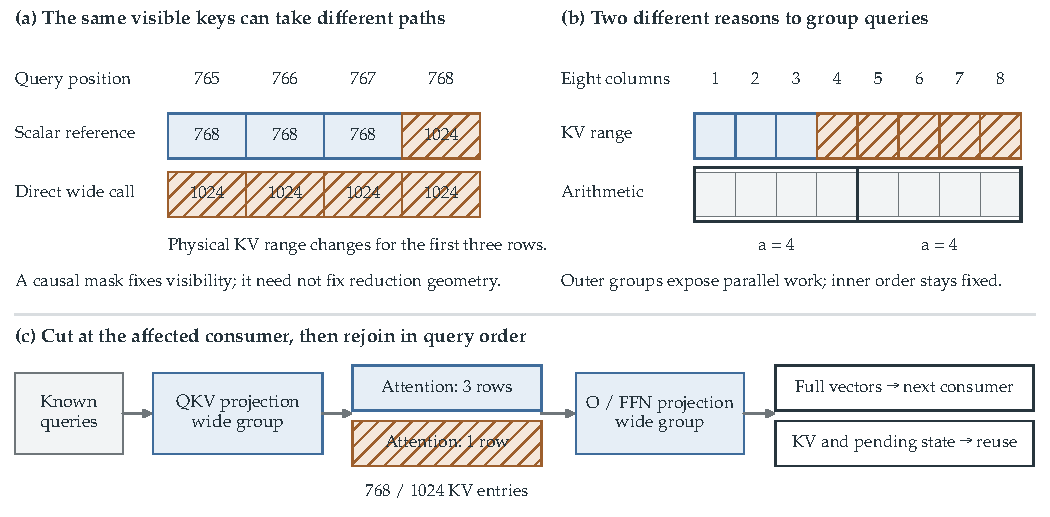
\includegraphics[width=\textwidth]{fig01_overview.pdf}
 \caption{Retain each group's numerical path while reorganizing execution across groups. (a) Four known queries cross a physical KV boundary. (b) Whole-call cuts divide surrounding projections; local cuts retain one four-column projection group while splitting attention. The backend must preserve the reference for each employed one- to four-column path. (c) Owned outputs retain row order; accepting two proposals keeps KV through position 767, while the correction at 768 remains pending. (d) A separate eight-query prefill illustrates two four-column arithmetic groups and attention tiles of four, three and one. Conceptual diagram prepared with ChatGPT (OpenAI, GPT-6 Astra Pro) assistance; editable drawing code is supplied.}
 \label{fig:overview}
\end{figure*}

This organization reuses existing small-column kernels, packing, weight broadcasting and fixed reductions. Its contribution is the construction that combines their arithmetic requirements with physical attention ranges and downstream output/state obligations. Structural invariants make the row mapping and cut placement explicit; backend conditions state what must hold for the arithmetic; qualification checks those conditions' consequences in the evaluated implementations. A conditional composition argument connects the resulting operations to subsequent decoder calls.

The experiments separate the method's two mechanisms and the costs around them. The 32B mixed-quantization instance keeps one-column arithmetic and whole-call cuts, isolating independent-group scheduling. Against a backend scalar loop that already shares activation quantization, it reduces A5000 target-only resident-service time by 1.51\% (95\% paired-root interval: 1.23--1.79\%). Q8 factorials independently vary four-column projection packing and whole versus local attention cuts. Controlled Vulkan appends measure the benefit of crossing a physical boundary; natural requests measure how often that opportunity occurs. Width experiments then show how cheaper equal-work verification can coexist with higher service time when deeper speculation creates extra target and draft work.

The paper contributes:
\begin{enumerate}
 \item A construction for fixed-reference parallel execution that separates physical and arithmetic groups, locates attention cuts, and preserves requested outputs and successor state.
 \item Concrete scalar-column and four-column CUDA instances, together with a Vulkan local-cut study, that connect the construction to existing quantized kernels and fair controls.
 \item An explanation of performance through grouping opportunities and their costs, supported by strong-control comparisons, component attribution, application measurements and negative cases.
\end{enumerate}

\section{Parallel execution with a fixed reference}
\label{sec:method}

\subsection{Two grouping decisions}
Consider four known queries at positions 765--768. A scalar continuation path with a 256-entry KV padding unit exposes physical attention ranges of $[768,768,768,1024]$. Executing the queries together can expose 1024 entries to every query. The causal mask still hides the same future tokens, yet the attention kernel now receives a different physical problem. In the captured CUDA case, the visible operands and probability prefixes agree, and the additional probabilities are zero; changing the physical range alone reproduces the two different attention--value outputs~\cite{records}. A mask preserves mathematical visibility, but need not preserve the executed reduction.

Splitting the entire decoder into calls of three queries and one query restores the required ranges. It also splits projections and feed-forward work that need no such boundary. Our construction keeps the wider decoder graph and places the split inside attention. This is the first grouping decision: which queries can share a physical KV range? The second concerns arithmetic: which query columns can share an existing quantizer and reduction specialization? These groups need not coincide (Fig.~\ref{fig:overview}).

For example, a supported CUDA Q8 projection preserves the established four-column arithmetic while presenting several such groups as independent channels. The mixed Q4\_K/Q6\_K implementation instead retains one-column arithmetic. Neither choice follows from the weight format alone: activation representation, reduction organization, tensor strides and device placement also determine the result. Parallel work is exposed around those decisions rather than by changing them.

\subsection{Reference and consumer contract}
The reference is a particular deployment, denoted $R_d$. It fixes model and tokenizer bytes, input formatting, numerical modules, placement, cache types and capacity, prompt production, requested outputs, and sampling and stopping rules. A different device or numerical backend defines a different reference.

Let $O$ be the output rows requested by the consumer. For a materialized prefix $x$, let $z_i(x)$ be row $i$'s complete binary32 vocabulary vector, and let $K(x)$ contain active keys and values in canonical logical order. Let $s(x)$ record logical positions, the retained frontier, any emitted but unmaterialized token, and termination status. The compatibility target at the relevant boundaries is
\begin{equation}
 \begin{split}
 z_i^{F}(x)&\overset{\mathrm{bits}}{=}z_i^{R_d}(x),\quad i\in O,\\
 K^{F}(x)&\overset{\mathrm{bits}}{=}K^{R_d}(x),\qquad
 s^{F}(x)=s^{R_d}(x).
 \end{split}
 \label{eq:reference-contract}
\end{equation}
Unused cache storage is outside this relation. Token agreement is a consequence for the specified greedy consumer, not a substitute for the vector and state obligations. A vector omitted from $O$ must be excluded by the consumer before execution, rather than discarded after finding a discrepancy.

Speculative verification illustrates why this distinction matters. The target evaluates a seed and draft proposals, including prefixes that may later be rejected. Their requested vectors are compared with an independent reference following those same prefixes after the fixed prompt producer. A separate autonomous reference supplies the generated-token endpoint. This preserves the target's obligations without requiring the draft to reproduce the reference trajectory.

\subsection{Constructing compatible groups}
The construction takes an ordered sequence of known token rows, their positions and requested-output flags, the incoming cache, and backend-specific numerical requirements. It returns an execution organization and owned outputs in the original logical order. Backend analysis supplies the numerical requirements; the planner does not discover equivalent kernels automatically.

For each row $i$, determine the physical extent $e_i$ that its reference call would expose. In the admitted dense, nonwrapping cache, with padding unit $P$, capacity $C$, and zero-based position $p_i$, this is
\begin{equation}
 e_i=\min\!\left(C,\max\!\left(P,
 P\left\lceil\frac{p_i+1}{P}\right\rceil\right)\right).
 \label{eq:physical-extent}
\end{equation}
The implementation obtains the padding and cache metadata from the native engine and checks the append mapping. It retains producer-specific behavior when a prompt phase uses a different reference schedule.

A \emph{physical group} is an adjacent run with the same extent and compatible attention descriptor, including relevant data types, layouts and dispatch conditions. Rows remain in their original order. Each run is tiled to the admitted attention width. A whole-call implementation, \textsc{Simple}, executes these groups as separate decoder calls. The \textsc{Local} implementation creates matching Q, K, V and mask views inside attention, computes each tile, and concatenates its outputs in logical order. QKV projections and feed-forward operations remain in the enclosing wider graph. This changes where the boundary is paid, not the causal dependencies between tokens.

An \emph{arithmetic group} retains a qualified column width $a$ and its numerical specialization. With an activation matrix $X\in\mathbb{R}^{K\times q}$, separate complete groups from the tail before taking the grouped view:
\begin{equation}
 \begin{split}
 X[K,q]&=[X_{\mathrm{full}}[K,ag]\;X_{\mathrm{tail}}[K,r]],\\
 X_{\mathrm{full}}[K,ag]&\longrightarrow X_{\mathrm{full}}[K,a,g],\\
 q&=ag+r,\qquad 0\le r<a.
 \end{split}
 \label{eq:arithmetic-groups}
\end{equation}
The outer dimension exposes independent groups to the existing backend while the inner width remains $a$; a tail uses an admitted smaller width. The weight tensor is broadcast across groups. Preserving a shape alone is insufficient: the selected kernel must retain the required activation quantization, inner reduction, strides and placement. Each deployment binds these choices to a fixed implementation; qualification checks the resulting outputs and state for the reported cases.

The reusable construction therefore has four steps:
\begin{enumerate}
 \item Bind the producer, incoming state, consumer outputs and backend numerical behavior.
 \item Derive each row's physical extent and partition the attention work at changes in extent or numerical descriptor.
 \item Retain the admitted inner arithmetic while exposing independent outer groups; keep extent-independent work outside local attention cuts.
 \item Copy requested outputs into row-owned storage, then commit the accepted state and logical frontier together.
\end{enumerate}
Equal-descriptor runs minimize the number of adjacent groups under those equality and width constraints. They do not minimize end-to-end latency: local views, launches, concatenation and output ownership all incur costs. The measured comparison between \textsc{Simple} and \textsc{Local} determines whether retaining wider work repays those costs.

\subsection{Why the construction composes}
The argument is conditional on three obligations: the incoming producer state satisfies Eq.~\ref{eq:reference-contract}; each admitted operator organization preserves its reference values and state effects; and the consumer receives the required outputs with the same commit semantics. Under these conditions, induction over the dependency graph preserves each intermediate required by subsequent operations. Physical views retain the reference operands and arithmetic, row-wise reconstruction retains output identity, and state updates retain the active prefix. Applying the same argument at successive commit boundaries preserves continuation.

Output ownership is essential to the last step. A later native call can reuse an earlier output buffer, while speculative acceptance can select an earlier row as the retained frontier. The executor therefore copies every requested vector before another group can overwrite its storage. It trims rejected KV entries and records a correction or bonus token as pending until that token is actually materialized. A generation limit or end-of-generation token can stop execution in this pending state.

This argument explains the obligations that an implementation must discharge. The experiments test the contract at their reported cases and boundaries; the argument is not an all-input proof of the native kernels. The methodological contribution is the separation of physical and arithmetic grouping, local placement of the resulting cuts, and composition through an explicit consumer contract. Packing, fixed reductions, weight broadcasting and existing small-column kernels remain reusable components of the construction~\cite{loop4code}.

\section{Implementation}
\label{sec:implementation}

\subsection{Two method instances and their controls}
We implement the construction in modified llama.cpp paths~\cite{records}. The phase executor owns a resident target context with a dense, contiguous, nonwrapping sequence and F16 keys and values. A backend-neutral planner preserves ordered rows, physical extents and requested-output flags; native adapters supply numerical descriptors and operations. The CUDA instance uses causal, non-Flash attention for the supported Llama and Qwen architectures.

For Q8 projections, full arithmetic groups have $a=4$. The packed path retains the existing small-column arithmetic~\cite{loop4code}, presents complete groups as channels, and restores column order afterward. The \emph{backend-loop4} control already quantizes the wide activation once before invoking four-column and tail kernels. The comparison therefore tests execution organization beyond shared quantization. Cross-group packing requires at least eight known rows. In the $k=3$ speculative applications, target verification has four rows, so this packing opportunity occurs in wider prefill work. The \Simple/\Local{} factor separately controls placement of the physical attention cuts.

The 32B mixed Q4\_K/Q6\_K instance instead uses $a=1$ and whole-graph cuts. B shares activation quantization and loops over scalar backend projections; C presents a $[K,1,q]$ view and reshapes the result. Both retain the one-column dot-product specialization. The S3 C/B comparison consequently measures scheduling of independent scalar groups, distinct from the Q8 \Local-plus-packed combination. The weaker G control performs scalar slicing at graph level.

The Vulkan instance retains F32 activations where the scalar reference uses F32, together with the required attention extent and layout. It provides a separate implementation of the grouping principle, with its own numerical reference and controlled append measurements.

\subsection{Output ownership, reuse and implementation coverage}
After each native call, the executor synchronizes and copies requested vocabulary vectors into storage indexed by logical row. It then checks the physical append endpoint. This preserves an earlier accepted row when subsequent calls reuse native output buffers. Planning uses native metadata without reference replay or KV export.

Graph reuse compares the numerical policy, complete per-row extent vector, relevant head-normalization and rotary-placement choices, and the engine's topology and output-count conditions. Requested row indices are refreshed as inputs. A mismatch rebuilds the graph. The deployment fixes additional numerical modules and model choices; the frontend's cache-type tag alone does not encode them all.

Online admission checks the supported cache and output reserve. Marked backend-loop4 operators additionally check descriptors, actual device residency and dispatch constraints. Packed nodes use ordinary backend dispatch and do not inherit every marker check; their arithmetic evidence comes from deployment-specific qualification. Capture runs collect selected operators, full vectors and native state for offline comparison, while clean service timings exclude those observers. The supplement maps these mechanisms to the actual source paths.

A failed target group poisons its context. The published command-line worker contains other failures by terminating, rather than recovering a partially updated service transaction. Detailed failure coverage is in the supplement. The method's state-commit argument concerns successful admitted executions; a reusable service library would also need transaction-wide invalidation on failure.

\section{Evaluation design}
\label{sec:eval}

\subsection{Questions, deployments and controls}
The experiments follow the construction from numerical mechanism to service value. A range intervention tests why physical grouping matters. The 32B study isolates scheduling across scalar arithmetic groups; the Q8 factorials separately vary projection packing and cut placement. Controlled appends and natural requests test how often local cuts remove useful work. Complete applications then account for draft execution and the work induced by a speculative policy.

The implementations run on an RTX A5000 with Linux/CUDA, an RTX 5070 Ti Laptop GPU with Windows/CUDA, and an Intel Arc B570 with Vulkan. Each deployment has its own reference. Resident model studies use a single dense, nonwrapping sequence, F16 keys and values, greedy generation, and non-Flash causal attention. The single-request A5000 panels use capacity 1024; the two-turn resident pilot uses 4096. Controlled Vulkan appends cover both capacities. Models come from the Qwen3, Llama and SmolLM2 families~\cite{qwen3,llama3,smol}. Table~\ref{tab:design} maps each experiment to the method component it exercises. Frozen sources, qualification coverage and complete numerical inputs accompany the supplement~\cite{records}.

\begin{table*}[t]
\centering\small
\caption{Method instances and the questions they test. Here $a$ is the projection arithmetic-group width and $q$ is the number of known target rows. A root is a task input; its repeated observations stay together in resampling. The Qwen Q8 service and factorial panels reuse the same 16 roots. Each row retains its own reference, experimental unit and clock.}
\label{tab:design}
\begin{tabularx}{\textwidth}{@{}p{3.1cm}p{3.8cm}p{3.5cm}Y@{}}
\toprule
Instance / question & Grouping and cut placement & Comparison & Units and measurement boundary\\
\midrule
32B scheduling increment; A5000, mixed Q4\_K/Q6\_K & $a=1$; whole-graph cuts fixed; target-only & G: graph scalar loop; B: shared quantization + backend scalar loop; C: independent scalar groups & 12 roots $\times$ 4 rounds; 144 measured and 144 warmup requests; resident service\\
Q8 component attribution; A5000, Qwen3-8B/14B & $a=4$; \Simple/\Local{} $\times$ backend-loop4/packed & Four-arm factorial; draft policy fixed; $q\le4$ in verification, wider prefill packs groups & 16 roots $\times$ 4 balanced rows per model; 256 measured requests; resident service\\
Controlled boundary opportunity; B570, SmolLM2 & Reference-compatible F32 path; $q=2,4,32$; whole/local cuts & Matched crossing and inside appends & 12 fixed cells, 3 paired repeats; prepared-state append, excluding state preparation\\
Complete Q8 application; A5000, Qwen3-8B/14B, Llama-8B & $a=4$; full draft and target execution & Four target-only controls and two speculative paths; same-draft increment also reported & 16/16/12 roots $\times$ 4 sessions; 384/384/288 measured requests; resident and worker clocks\\
Natural two-turn pilot; A5000, Qwen3-8B Q8 & Capacity 4096; whole/local cuts; backend-loop4 fixed; no draft & Common canonical-history repair; local placement is the treatment & 2 development conversations $\times$ 2 rounds $\times$ 2 arms; complete two-turn embedded service\\
Numerical migration alternative; RTX laptop, Qwen3-8B Q8 & $q=8$; old packed B versus modern U & Quantizer and projection contract change together & 1 captured input, 12 pairs per boundary; extracted operator, excluding allocation, copies and checks\\
\bottomrule
\end{tabularx}
\end{table*}

In the Q8 panels, W and L denote \Simple{} whole-graph cuts and \Local{} attention cuts, while L4 and P denote backend-loop4 and packed projections. M denotes target-only generation, which loads no draft model. D4 denotes speculative generation with draft prefill microbatch four; the proposal count is $k=3$. Thus, D4 is a draft setting, $q$ counts target query rows, and Q8\_0 is a weight format. Qwen targets use a Qwen3-0.6B draft; the Llama pair is Meta-Llama-3.1-8B-Instruct with Llama-3.2-1B-Instruct. All arms receive the same applicable residency, graph reuse and numerical fixes.

The 32B panel isolates scheduling across groups without a draft or a local-cut treatment. It fixes whole-graph attention cuts, two CPU threads, context capacity 1024, target microbatch and output reserve 32, and disabled CUDA graphs. Its 12 new roots comprise six coding and six mathematics tasks, with 39--187 prompt tokens and a 128-token output cap. Each of 144 fresh workers performs an identical-root warmup followed by one formal request. G slices scalar projections at graph level; B shares activation quantization and loops over scalar backend calls; C exposes those scalar computations as channels. C/B is the primary method comparison. Its $a=1$ scalar-loop B is distinct from the $a=4$ backend-loop4 control in the Q8 factorials.

The Qwen Q8 studies use pinned APPS and MATH inputs~\cite{apps,math}, reusing task identities across sizes and platforms but establishing each deployment's reference separately. Llama's 12 roots were selected after excluding prior project exposure. The multi-turn pilot uses two development conversations from OpenAssistant~\cite{oasst}. These fixed workloads support deployment-specific estimates; model size is not a substitute for independent workload sampling.

\subsection{Qualification and clocks}
Offline qualification compares requested full vocabulary vectors and active KV entries in canonical logical order. Forced-prefix reference runs check speculative branches; an autonomous reference checks emitted tokens and stopping. Across qualification campaigns, the checked cases include prefill, continuation, boundary crossing, rejection, trim, pending tokens, termination and reset. Clean timing disables heavy observers and retains the corresponding endpoint, identity and execution-trace checks. The supplement associates observation scope with each implementation; it does not treat a clean endpoint check as a new full-state comparison.

Resident-service time includes reset, planning, target and applicable draft work, sampling, state bookkeeping, synchronization and requested-output copies. It excludes model loading, context construction and diagnostic export. The two-turn pilot additionally includes history rendering, tokenization, controller transport and durable per-decode accounting in its frozen host adapter. Worker clocks include initialization and primers and are reported separately. These are embedded request paths, without concurrent network serving or queueing. Prepared-state appends and extracted GPU-event operators have narrower boundaries, stated in their captions.

\subsection{Estimands and uncertainty}
For the 32B primary comparison, we average paired log time ratios over four rounds within each root and then equally over 12 roots:
\begin{equation}
 \rho_{C/B}=\exp\!\left(\frac{1}{12}\sum_{r=1}^{12}
 \frac{1}{4}\sum_{s=1}^{4}\log\frac{t_{rsC}}{t_{rsB}}\right).
 \label{eq:s3-estimand}
\end{equation}
The paired-root bootstrap resamples six coding roots and six mathematics roots within their strata, preserving their equal contribution. It uses 20,000 draws and a 95\% percentile interval for C/B; the two secondary G comparisons use 97.5\% intervals. All repetitions and arms of a sampled root remain together. The ratio of pooled totals is a different estimand and is identified separately.

A5000 Q8 service and factorial effects use the ratio of total service time, $\sum_{r,s}t_{rsA}/\sum_{r,s}t_{rsB}$. Their 10,000-draw paired-root bootstrap uses 99\% intervals for the five-comparison family. The interaction is an equal-root geometric ratio of component ratios. The factorials use four-arm Williams orders; six-arm service orders have partial balance, and the earlier 8B speculative pair retains its fixed order. Intervals condition on the observed sessions and tested roots. Three-repeat structural cells show their paired ranges; the two-episode pilot has no population interval. All time reductions are $100(1-\rho)$, not throughput increases.

The accompanying CPU scripts reaggregate the published rows and reconstruct the figures. Phase totals are descriptive sums of the same measured requests, kept separate from root-level inference. A supplementary leave-one-root-out check is explicitly post hoc and leaves the primary estimator and interval unchanged. ChatGPT (OpenAI, GPT-6 Astra Pro, accessed 13 November 2026) assisted manuscript preparation, CPU analysis and visualization code, and the conceptual diagrams. Numerical plots use the identified measurements; this revision adds no model execution.

\section{Results}
\label{sec:results}

\subsection{Physical range is part of the numerical problem}
\label{sec:range-result}
The CUDA diagnostic holds the query width at one and intervenes on the physical range supplied to attention--value multiplication. Cropping the wider execution from 1024 to 768 entries reproduces the shorter-reference output; padding the shorter execution to 1024 reproduces the wider output (Fig.~\ref{fig:extent}). Visible operands and probability prefixes agree in the captured case, and the added probabilities are zero. The bidirectional intervention supports the physical-range mechanism at that operator. It observes the complete attention--value output, rather than inferring equality from the eventual argmax.

\begin{figure*}[t]
 \centering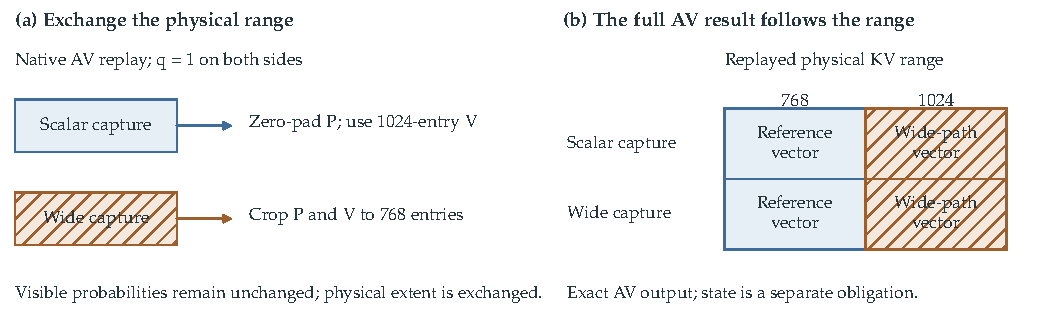
\includegraphics[width=\textwidth]{fig02_extent.pdf}
 \caption{A physical-range intervention changes the attention--value result. The captured CUDA comparison fixes a one-query consumer and tests 768- and 1024-entry physical ranges. Cropping and padding reproduce the respective reference outputs while retaining the visible operands. The observations concern the complete output of this operator; they do not measure KV-state equivalence or service time. The separate Vulkan study changes layout and dispatch together with range and is therefore a joint repair, not an isolated range intervention. Data and intervention identities are in the accompanying figure manifest.}
 \label{fig:extent}
\end{figure*}

At its tested boundaries, the 32B strong-control qualification passes comparisons of full 151,936-entry vocabulary vectors and active F16 KV across 64 layers. These observations complement the construction's conditional argument. The supplement identifies the coverage and retained records for the other profiles. Its CPU counterexamples show why the output and state obligations are necessary: matching argmax values can coexist with changed full vectors, serialized state and forced continuation.

\subsection{Independent groups improve on shared quantization}
\label{sec:strong-result}
Figure~\ref{fig:strong} shows the strongest direct service comparison for the execution organization. On the 32B target-only deployment, C/B is 0.984864, with a 95\% paired-root interval of [0.982148, 0.987721]. The corresponding reduction is 1.51\% [1.23\%, 1.79\%]. All 48 measured paired requests favor C, but the inferential unit is the 12 roots, not the 48 repeats.

\begin{figure*}[t]
 \centering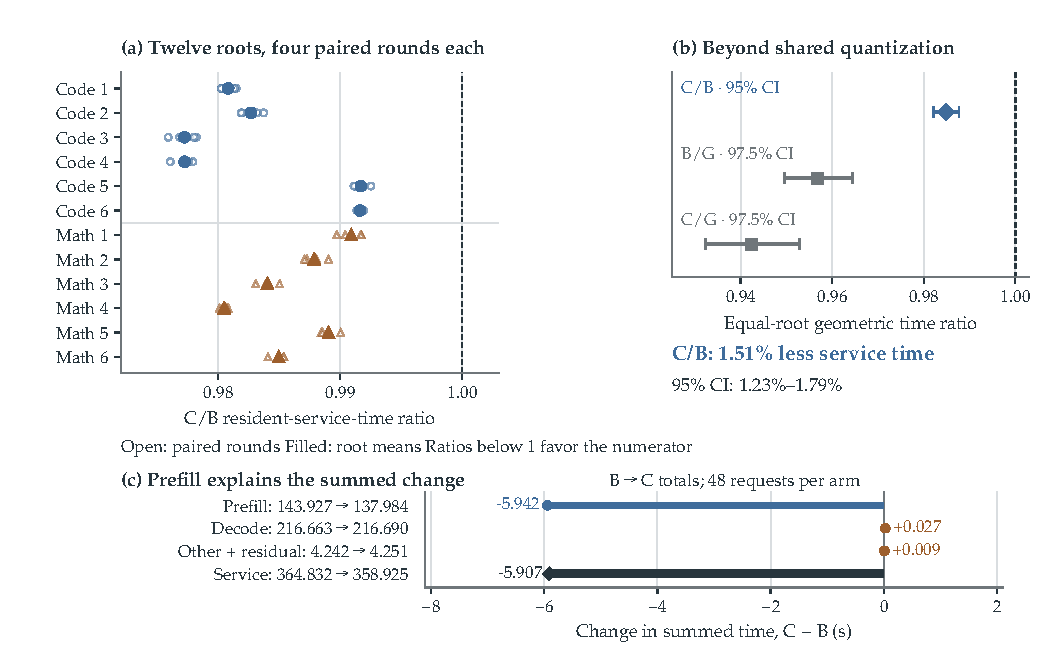
\includegraphics[width=\textwidth]{fig03_strong_baseline.pdf}
 \caption{The incremental service benefit beyond a strong same-contract control. A5000, Qwen3-32B-Q4\_K\_M, target-only generation, fixed whole-graph cuts. Root points average paired log ratios over four rounds. The primary C/B summary weights 12 roots equally and uses a 95\% paired-root interval stratified by coding and mathematics roots. Secondary B/G and C/G summaries use 97.5\% intervals. B shares activation quantization and invokes scalar backend projections; C schedules those scalar computations as independent channels. G is the weaker graph-level scalar loop. The resident timer includes reset and output ownership but excludes loading and diagnostic capture.}
 \label{fig:strong}
\end{figure*}

The weaker control explains why baseline choice matters. B/G is 0.956855 and C/G is 0.942372. Much of the advantage over G is already obtained by moving the scalar loop into the backend and sharing quantization. C/B isolates the remaining organization change. Across the 48 requests, B and C take 364.832 and 358.925\,s in total; their pooled ratio, 0.983809, differs from Eq.~\ref{eq:s3-estimand}. Prefill falls from 143.927 to 137.984\,s, while decode is effectively unchanged at 216.663 and 216.690\,s. This localization agrees with the opportunity to group known prompt rows. The result establishes a measurable compatibility-preserving increment in this deployment, without assigning draft-model benefits to it.

\subsection{Packing and local cuts have different opportunities}
\label{sec:factor-result}
The Q8 factorials fix the draft policy and cross cut placement with projection organization (Fig.~\ref{fig:factorial}). Packing reduces service by 1.64\% with \Simple{} and 1.56\% with \Local{} at 8B, and by 0.99\% and 0.80\% at 14B. Their backend-loop4 controls already share activation quantization, so these contrasts measure the remaining packed-group increment.

\begin{figure*}[t]
 \centering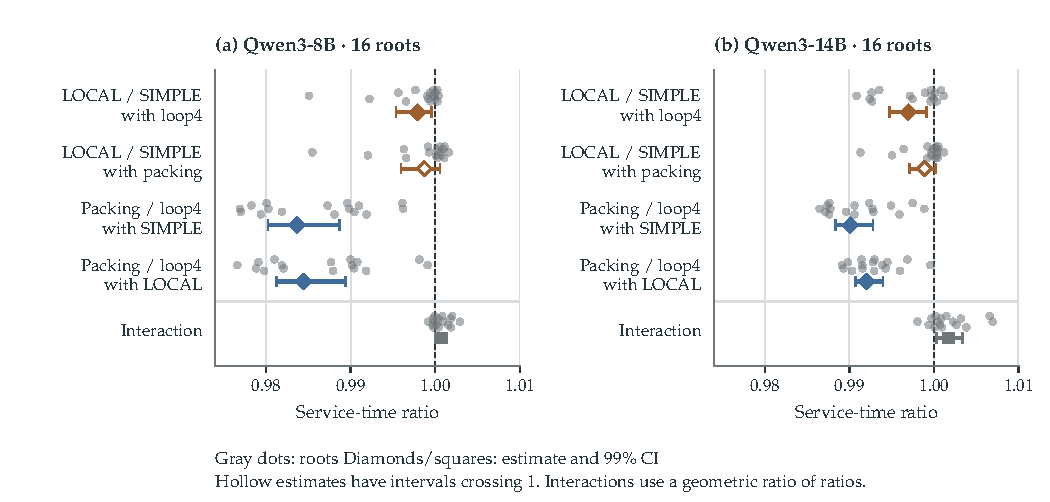
\includegraphics[width=\textwidth]{fig04_factorial.pdf}
 \caption{Separating the two execution changes. Balanced A5000 Q8 factorials fix draft prefill microbatch four and proposal count three. Faint points show individual root ratios; summary markers show ratios of total resident-service time with 99\% paired-root intervals from the five-comparison family. Projection contrasts hold cut placement fixed; cut contrasts hold projection fixed. The interaction summary is an equal-root geometric ratio of ratios. The two models share 16 task roots and are separate measurements. Intervals spanning one are visibly retained.}
 \label{fig:factorial}
\end{figure*}

Local cuts reduce service by 0.21\% and 0.30\% at fixed loop4. At fixed packing, the reductions are 0.13\% and 0.11\%, with both intervals containing zero reduction. The equal-root interactions are 1.000696 and 1.001703, indicating slight attenuation when both components are applied. At $k=3$, target verification has at most four queries, so it does not enter the multi-group Q8 packing route. Execution records place that route in prefill. The components consequently address different opportunities even within one request.

\subsection{Boundary geometry explains the local-cut results}
\label{sec:geometry-result}
In the natural 8B factorial, 20 of 2,224 logical verification cycles require an additional whole-graph split. \Simple{} uses 2,244 graphs and \Local{} 2,224 for the same target rows: just 0.899\% of cycles present that opportunity. The controlled B570 appends make the opportunity explicit (Fig.~\ref{fig:geometry}). A crossing starts one row before a physical boundary and forces the whole-graph split $1+(q-1)$, for $q=2,4,32$. Across capacities 1024 and 4096, local execution takes 20.34--44.68\% less append time in these cells. Matched inside controls take 0.43--3.74\% more time. Three paired observations per cell show repeat variation, not a workload confidence interval.

\begin{figure*}[t]
 \centering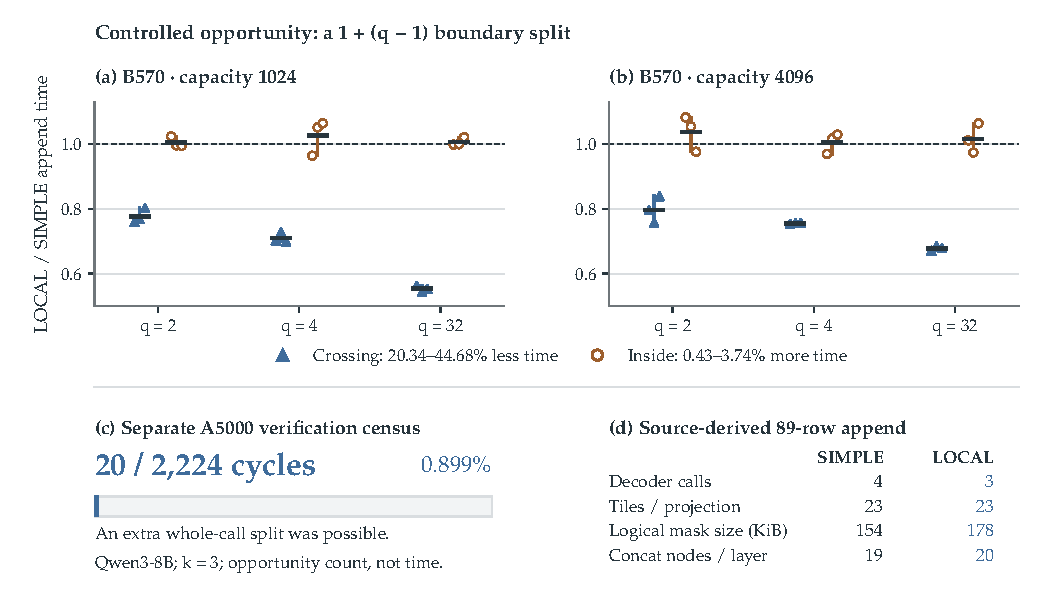
\includegraphics[width=\textwidth]{fig06_geometry.pdf}
 \caption{Local cuts help when they retain enough surrounding work. The opportunity count on A5000 is shown separately from B570 operation timings. B570 points compare \Local/\Simple{} append time at fixed $q$ and capacity; crossing triangles and inside circles use distinct shapes and fills. Ranges are the minimum and maximum of three paired repeats. The prepared-state timer includes binding, decode, synchronization and requested-output copying, and excludes state preparation. Capacity and prefix region change together between the two capacity panels. Earlier $16+16$ crossings, including reversals, are retained in the supplement.}
 \label{fig:geometry}
\end{figure*}

Crossing alone is not sufficient. Earlier $q=32$ cells with a $16+16$ whole-graph split include cases favoring \Simple{}. In the natural multi-turn pilot, the four paired episode ratios are 1.0997, 1.0024, 1.0886 and 0.9888 (Table~\ref{tab:natural}). Across the eight timed episodes, \Local{} takes 37.921\,s versus 36.385\,s for \Simple{}, a descriptive ratio of 1.04220. The pilot therefore provides no observed local-cut service improvement; two development conversations cannot establish a population ranking.

\begin{table}[t]
\centering\small
\caption{Natural multi-turn pilot: \Local/\Simple{} resident-service ratios. Packing and the request protocol are fixed. Rows are two rounds of each development episode, not four independent tasks. No confidence interval is inferred.}
\label{tab:natural}
\begin{tabular}{@{}lrr@{}}\toprule
Episode & Round 1 & Round 2\\\midrule
Development conversation A & 1.0997 & 1.0024\\
Development conversation B & 1.0886 & 0.9888\\\midrule
Pooled ratio & \multicolumn{2}{r}{1.04220}\\\bottomrule
\end{tabular}
\end{table}

The pilot's complete calls fall from 1,072 to 1,070. A separate source-derived plan for one proposed 89-row supplied-history append finds four versus three decoder calls but the same 23 ordered projection tiles. Fewer outer calls can therefore leave the principal arithmetic work unchanged. These observations identify limits on the natural-request opportunity: local placement avoids some graph fragmentation, while view construction, attention launches and concatenation remain real costs.

\subsection{Application gains are larger than the method increment}
\label{sec:application-result}
The complete Q8 speculative applications improve on all four target-only controls (Fig.~\ref{fig:application}). Against the fastest measured fixed M, \Local-packed D4 reduces resident service by 17.21\% for Qwen3-8B, 25.54\% for Qwen3-14B, and 11.52\% for Llama-8B. Their adjusted 99\% intervals are [11.17\%, 24.61\%], [18.21\%, 34.89\%], and [4.33\%, 20.95\%], respectively. These comparisons include the draft and the complete verification application. Against \Simple-loop4 with the same D4 policy, the corresponding increments are 2.01\%, 1.08\% and 1.56\%.

\begin{figure*}[t]
 \centering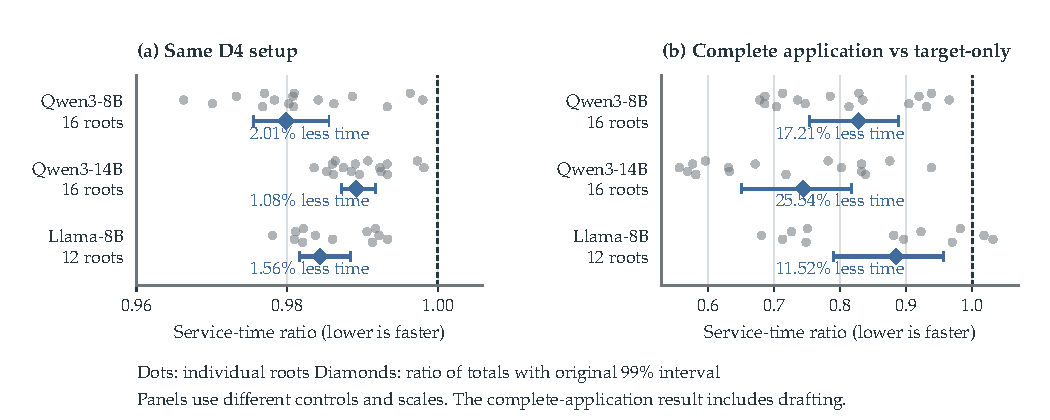
\includegraphics[width=\textwidth]{fig05_application.pdf}
 \caption{Application value and execution increment answer different questions. Panel (a) compares \Local-packed D4 with \Simple-loop4 D4 under the same draft policy; panel (b) compares it with the fastest measured fixed target-only control. Points retain root heterogeneity; summaries are ratios of total resident-service time with 99\% paired-root intervals. Qwen panels use the same 16 roots; Llama uses 12 separately selected roots. All fixed target-only comparisons are retained in the supplement, so choosing the fastest measured M does not replace the prespecified control family. The larger application reductions include speculative decoding.}
 \label{fig:application}
\end{figure*}

Initialization can change the decision. For the 14B request burst, worker time including loading, integrity checks and primers falls from 662.546\,s for W-P-M to 594.559\,s for \Local-packed D4. Llama's resident requests improve, yet its short worker workload favors target-only execution: the fastest M worker takes 355.730\,s versus 368.822\,s for \Local-packed D4. The earlier 32B panel instead favors ordinary grouped generation; grouped D4 takes about 14\% more resident time. A B570 pilot likewise favors target-only generation despite fewer target graphs in the speculative path. The supplement retains these complete cost accounts.

Wider execution also needs a workload distinction. A Windows RTX equal-work diagnostic makes one $q=8$ call 3.94--11.91\% cheaper than two $q=4$ calls from the same state with the same eight known tokens and requested outputs. In live generation, increasing proposals from $k=3$ to $k=7$ raises service time by 13.58--14.59\% across the four methods. For the same 11,472 emitted tokens, verification cycles fall from 3,504 to 2,296, but verified rows rise from 14,016 to 18,368 and draft proposals from 10,512 to 16,072. Avoiding launches does not repay the extra unconsumed work.

\subsection{A modern backend is a different engineering choice}
\label{sec:modern-result}
A recent upstream llama.cpp few-row implementation~\cite{llama_cpp_fewrow} provides a useful alternative. On one captured Qwen3-8B Q8 input with $K=N=4096$ and $q=8$, the ratio of upstream U to the extracted legacy packed Q8 operator B is 0.612924, with a 95\% paired-repeat interval [0.607906, 0.618665]. The 38.7\% reduction belongs to that operator comparison. U uses a different quantization and projection contract: 32,766 of 32,768 output bit patterns differ from the legacy reference. The preceding attempt to qualify U against the earlier strict CPU-round-to-nearest oracle for the upstream path failed and produced no timing under that oracle. The later comparison declares U's own contract instead.

This result favors considering a numerical migration when exact compatibility is unnecessary. It does not measure a complete default upstream backend: that backend's qualification and paired service timing have not been run. Two legacy-compatible extracted candidates also fail to improve the strong control, with complete-operator ratios 1.1264 and 1.0261 in their separate sessions. The available measurements compare operator choices; they leave the complete-backend service comparison open.

\Needspace{9\baselineskip}
\section{Related work}
\label{sec:related}

\paragraph{Matching an existing numerical reference.}
Yang et al. reconstruct the arithmetic of cuBLAS kernels and enforce bitwise behavior through compiler transformations and static verification~\cite{taming}. Their computation descriptors separate reduction structure from scheduling: output tiling and pipelining can change when each output retains its arithmetic. Their reconstruction targets matrix multiplication; attention receives a theoretical treatment whose implementation remains open. Our construction adds query-specific physical KV views, local attention cuts and successor-state obligations within a quantized decoder.

\paragraph{Batch invariance and fixed scheduling.}
He and Thinking Machines Lab construct batch-invariant normalization, matrix multiplication and attention~\cite{thinkingmachines}. Their attention analysis shows why separating cached KV entries from newly computed entries can change reduction grouping. Fixed reductions and the numerical significance of cache boundaries are therefore established ideas. Here, the selected reference supplies each query's physical extent, including initialized entries outside its logical causal prefix; the executor retains that extent where the attention computation requires it.

CoRun fixes the execution context through isolated prefill, padded fixed-shape decode, position-invariant kernels and request-specific sampling state~\cite{corun}. That policy preserves repeatable request-local arithmetic while allowing co-runners and batch slots to change. Our input is a previously selected numerical deployment, which can prescribe different physical ranges for adjacent queries. Local cuts honor those differences while surrounding compatible work remains grouped.

\paragraph{Outputs, persistent state and repair.}
Vosti specifies deterministic inference through request outputs and verifies engine invariants together with kernel contracts~\cite{vosti}. Its KV invariant covers live and retained reusable entries, tying each value to its logical token prefix. Its engine proof depends on imported kernel contracts, which a separate verifier discharges for supported kernels. Our conditional argument uses output and state obligations to compose an execution transformation in an existing implementation; finite qualification supplies the empirical coverage reported here.

LLM-42 permits dynamic batching on a fast path, then uses fixed-shape verification to commit a consistent prefix or roll back~\cite{llm42}. Even when tokens agree, it replaces the fast path's KV entries with verifier-produced entries. Our transformation instead preserves the selected target path before consumer commit. It adds no separate numerical repair pass; ordinary speculative token acceptance still belongs to the consumer.

\paragraph{Quantized kernels and inference optimization.}
The implementation inherits deterministic quantized operations and four-column execution from \texttt{llama\_reproducible}~\cite{loop4code}. Modern \texttt{llama.cpp} uses integer tensor-core operations, asynchronous copies and reuse across column groups in its few-row quantized matrix multiplication~\cite{llama_cpp_fewrow}. These are existing optimization mechanisms. Our evaluation separates reorganization under the selected reference from adoption of a modern operator with a different quantizer and projection arithmetic. FlashAttention reduces attention memory traffic through tiling~\cite{flashattention}; FlashInfer supports heterogeneous KV layouts and load-balanced execution~\cite{flashinfer}. Fixed-reference compatibility adds an implementation-level numerical condition to those optimization goals.

\paragraph{Speculative decoding.}
Speculative decoding and sampling verify several draft tokens together to amortize target work~\cite{leviathan2023,chen2023}. Their distribution-preservation arguments concern the sampling algorithm. Liu et al. adapt verification effort to candidate uncertainty~\cite{liu2026heterospec}. Our method organizes already selected query tokens under a numerical reference. We therefore separate complete speculative-application results from factorials that fix the draft policy and isolate projection packing, local cuts and their interaction.

\section{Discussion and limitations}
\label{sec:discussion}

\subsection{When retaining a reference is worth the cost}
The fixed reference is an application constraint, not a universal performance objective. It can isolate scheduling changes during regression testing, permit exact replay from stored state, or support a component migration while its consumer remains unchanged. In such settings, a small execution improvement can be useful because the optimized path preserves the expected numerical interface. The 32B result shows that this option has measurable value beyond a strong implementation control. It does not establish a production return on maintenance effort, energy savings, or a general preference for the legacy backend.

A deployment free to change its numerical contract should evaluate that option directly. The modern extracted operator illustrates the possible benefit. A fair system decision would compare complete, appropriately qualified backends on the intended workload and include the cost of migration or compatibility. Our current evidence contains the legacy-compatible service comparison and the modern operator comparison, with different scopes; the missing full-backend comparison remains an open engineering decision rather than an assumed win for either choice.

\subsection{What transfers beyond this implementation}
The transferable object is the construction procedure: derive the physical and arithmetic constraints of a chosen reference, place the required cuts at the operations that depend on them, and check the consumer's outputs and successor state. It directs implementation and testing even when a backend uses different widths or cache layouts.

The implementation remains specialized. Its two projection widths and CUDA/Vulkan paths demonstrate instances of the construction, not automatic transfer to arbitrary quantizers, paged or sliding caches, mixed-device partitions, Flash attention, concurrent sequences, or stochastic sampling. Adding such a path requires deriving its numerical descriptor, discharging its state obligations and qualifying its actual dispatch. The conditional composition argument helps identify those obligations; it does not replace that work. Likewise, existing batching and packing techniques supply components, so the contribution should be judged by the combined execution organization and the evidence explaining its costs.

\subsection{Why the negative results matter}
The results expose three distinct constraints on performance. A local cut has little value when a request seldom crosses the relevant physical boundary. Even at a crossing, preserving a wider graph may leave the same arithmetic tiles or incur enough attention overhead to lose. Finally, a more efficient fixed operation can still make an application slower when it induces additional draft and target work. These mechanisms explain the small factorial cut effect, the multi-turn pilot and the wider-speculation reversal without requiring a universal threshold for useful speedup.

The evidence is also limited by its sampling. Several studies reuse development roots, and the Qwen scales reuse input identities. Confidence intervals preserve root clustering and describe the stated sessions; they do not measure cross-machine, cross-day or population-wide variation. Structural cells and the two-episode pilot are descriptive. Workload identities, orders, clocks and uncertainty types therefore remain explicit in the figures and supplement.

\subsection{Reproducibility and implementation maturity}
Public timing rows support independent statistical reconstruction, and the source maps identify the code and public diagnostics behind each result. Some native records are company-restricted, and some temporary intermediates were pruned. Public summaries cannot substitute for unavailable original tensors. The present reconstruction checks published statistics and implementations without rerunning native qualification. The final archival deposit and any permitted restricted-access procedure require author confirmation.

The current command-line implementation also has a narrower recovery boundary than a persistent inference service. Target-group errors poison the context, while other failures terminate the worker. A reusable service library would need transaction-wide invalidation and explicit admission for the unsupported graph cases. These requirements concern deployment maturity; the measured service timer remains the complete resident request path in the stated worker.

\section{Conclusion}
A fixed numerical reference leaves freedom to organize parallel work across groups that retain their internal arithmetic. Separating physical KV ranges from arithmetic groups places attention cuts where they are required while keeping compatible surrounding computation grouped. Row-owned outputs, accepted-prefix trimming and pending-token bookkeeping preserve the information needed by subsequent consumers under the stated backend conditions.

On the evaluated A5000 Qwen3-32B deployment, independent scalar-group execution reduces target-only resident-service time by 1.51\% relative to a strong same-contract backend scalar-loop control that already shares activation quantization. This instance uses $a=1$ and whole-call cuts; its saving is concentrated in prefill while decode remains nearly unchanged. The component and application studies explain how service value emerges: compatible grouping opportunities must occur, the retained surrounding work must yield a saving, and that saving must exceed the additional organization and speculative work.

\section*{Data and code availability}
Implementation sources, public timing rows, numerical projections and reconstruction scripts are linked by fixed revisions in the supplementary material and accompanying source manifest~\cite{records}. The source package includes the inputs and scripts needed to reproduce the reported CPU statistics, tables and figures. Some underlying native logs and tensor records are company-restricted; selected temporary intermediates were pruned and are no longer available. Those records are not included in the public reconstruction. Original model weights are identified at their sources and are not redistributed with the paper.

\section*{Declaration of generative AI and AI-assisted technologies}
ChatGPT (OpenAI, GPT-6 Astra Pro, accessed 13 November 2026) assisted manuscript drafting and English editing, literature and code checks, CPU statistical analysis, visualization code, conceptual diagrams, and LaTeX layout review. Numerical figures were generated by scripts from the identified experimental records. Project records also report AI assistance in the earlier research-code workflow. During this revision, no model or GPU measurements were added, and the recorded experimental data were preserved.

\balance
\bibliographystyle{unsrtnat}
\bibliography{references}
\end{document}
